%%%%%%%%%%%%%%%%%%%%%%%%%%%%%%%%%%%%%%%%%%%%%%%%%%%%%%%%%%%%%%%%%%%%%%%%%%%%%%%%
% DRAFT SECTION FRAGMENT -- gradient analysis (Q0-Q6).  Written 2026-08-14.
% FOR OWNER REVIEW ONLY.  Nothing here has been merged into "main (1).tex".
%
% HOW TO USE THIS FILE
%   * Conventions follow "main (1).tex": ieeeconf, \S\ref{}, "$+2.0$\,pp",
%     \emph{} for first-use terms, honest-caveat comments inline.
%   * Drop-in as a new \section after \S\ref{sec:exp} (EXPERIMENTS), or demote
%     every \subsection below to \subsubsection and nest it inside \S\ref{sec:exp}.
%   * OVERLAP WARNING: \S4.4 of main.tex ("Why influence loses: a gradient-encoding
%     ceiling") already states the AUC-level version of claim (1) for *object
%     category*.  This section is the *experiment-level* version for the bandit's
%     own behavior-descriptor region, plus the absorption / prediction / positive-
%     control / weight-space / quality results that \S4.4 does not have.  If both
%     are kept, cut \S4.4 down to two sentences and forward-reference here, or the
%     paper says the same thing twice.  Related Work \S\ref{sec:related} para. 1
%     already promises "gated by gradient encoding" -- this section delivers it.
%   * FIGURE: add {gradient_analysis/} to \graphicspath in the preamble.
%   * At the END of this file: a comment block listing every claim NOT yet backed
%     by a completed experiment.  Read it before submitting.
%%%%%%%%%%%%%%%%%%%%%%%%%%%%%%%%%%%%%%%%%%%%%%%%%%%%%%%%%%%%%%%%%%%%%%%%%%%%%%%%

\section{WHY POOL SELECTION IS CLOSED: A GRADIENT-LEVEL DIAGNOSIS}
\label{sec:gradient}

\S\ref{sec:anticorr} established, behaviorally, that no way of re-selecting
existing demonstrations closed the residual gap. A behavioral null is weak
evidence: it is always answerable with ``run more seeds.'' This section replaces
it with a \emph{mechanism}. We measure, in the learner's own gradient space,
whether the distinction we are trying to select on is visible to the training
loss at all---and show it is not, that this is a property of the objective
rather than of our experimental design, and that one axis the loss \emph{can}
see is not the one selection methods have been targeting.

\subsection{Setup and terminology}
\label{sec:grad_setup}
All experiments below run on a frozen apparatus, so that every comparison
differs only in data. An \emph{arm} is a selection rule (e.g.\ ``draw only from
the diagnosed failure region''). A \emph{draw} is the concrete set of $B{=}200$
pool demonstrations an arm samples in a given round. A \emph{pull} is one
complete draw$\rightarrow$fine-tune$\rightarrow$evaluate cycle: the draw is
added to the fixed $400$-demonstration base set $\mathcal{D}_{\text{base}}$, the
policy is fine-tuned with the identical recipe (pi0 LoRA, $20{,}000$ steps,
batch $32$), and the result is rolled out. The \emph{branching checkpoint} is
$\pi_0$ at step $19{,}999$ of base training---the single shared starting point
every pull fine-tunes from, and therefore the only checkpoint at which an
\emph{a priori} selector could act. Evaluation uses a frozen set $E$ of $150$
saved scene states $\times\,3$ repeats ($450$ rollouts per evaluated
checkpoint), partitioned into three \emph{strata} of $50$ scene states each
(hard / mid / easy) by a frozen difficulty map fit before the study
(held-out AUC $0.629$); ``hard'' is the diagnosed failure region. Baseline
success on $E$ is $51.3\%$, and the per-pull noise floor, estimated from
null pulls that add no demonstrations at all ($+2.4$ and $-0.9$\,pp), is
$\sigma_e = 3.3$\,pp. \emph{Any single-pull difference below $\approx$$3.3$\,pp
is reported below as directional, never as an effect.}

Finally, a \emph{gate} is a cheap up-front test of whether a target distinction
is encoded in the training gradient at all. We compute per-demonstration LoRA
gradients ($\approx$$50$M dimensions, $K{=}8$ frames per demonstration),
sparse-JL sketch them to $2048$ dimensions (sketch fidelity: true-cosine vs.\
sketch-cosine correlation $0.942$), and score two statistics: the
\emph{best-single-SVD-mode AUC} (unsupervised: does any principal direction of
the gradient cloud separate the two label groups?) and a \emph{split-half
contrast AUC} (supervised: fit a contrast direction on half the demonstrations,
score the held-out half). Because the first statistic maximizes over modes, it
must be read against its own label-shuffled null floor, which sits near $0.60$
at these sample sizes---a point we belabor because reading $0.577$ as
``slightly above chance'' inverts the conclusion.

\subsection{The gate fails: the flow-matching gradient does not encode the
failure region}
\label{sec:grad_q0}
At the branching checkpoint we gated the diagnosed failure region
(a behavior-descriptor cluster of tall-vessel grasp failures) using $120$
in-region against $120$ out-of-region pool demonstrations, the out-set
stratified over the remaining regions. The gate fails on both statistics: the
best-single-SVD-mode AUC is $0.577$, \emph{below} its own label-shuffled null
floor (mean $0.598$, max $0.622$ over $8$ shuffles), and the supervised
split-half contrast reaches only $0.572$ (shuffled labels $0.501$; a random
direction $0.536$). Whitening out the top-$10$ shared modes lifts the
split-half score to $0.660$, still far under the $\approx$$0.70$ bar that
prior validations require, and whitening further collapses it
($0.53$ at $k{=}25$, $0.35$ at $k{=}50$).

The consequence for selection is direct. Scoring each of the eight
round-3/4 draws ($8\times200$ demonstrations) against the fitted region
direction, a $100\%$ in-region draw has mean cosine $0.024$ while a
uniformly random draw---about $23\%$ in-region---has $0.019$. Both sit under a
shared ``generic pick-and-place'' component of $\approx$$0.20$, roughly ten
times larger than any region-specific residual. In gradient space, the treatment
and the control are the same treatment: at $B{=}200$, two draws are
near-interchangeable inputs to the optimizer, so data \emph{composition} cannot
matter at the region level---only data \emph{quantity}.

The instrument is not blind. On the same run, demonstrations the model had
already trained on (the base set) show mean gradient norm $0.554$ against
$3.136$ for unseen pool demonstrations---a $6\times$ absorption gap. The
pipeline detects real training structure; the flat region signal is an absence,
not an insensitivity.

\subsection{The demonstrations were absorbed---they do not contain the skill}
\label{sec:grad_q2}
A null could still mean the fine-tune never digested its data. It did.
Recomputing per-demonstration gradient norms along six fine-tune trajectories
(4 checkpoints $\times$ 360 demonstrations each: the pull's own $200$, $100$
never-trained pool controls, $60$ base-set demonstrations), a draw's own
demonstrations collapse from $3.1$--$3.3$ at the branching checkpoint to
$0.38$--$0.41$ by step $5000$ of $20{,}000$---indistinguishable from the
always-trained base set measured at the same checkpoint
($0.36$--$0.40$)---and stay flat thereafter. The arm trained on $200$ in-region
demonstrations absorbed them completely while its own hard stratum never
reliably moved. The failure is not under-training: \emph{the demonstrations do
not contain the missing skill}.

Two further readings come free. First, the recipe specializes hard after step
$5000$: never-seen control demonstrations, well fit at step $5000$
($0.43$--$0.47$), climb monotonically back toward the pre-fine-tune level
($1.11$--$1.17$, $1.67$--$1.72$, $2.37$--$2.45$ at steps $10{,}000$, $15{,}000$,
$19{,}999$) while own-draw norms stay flat. Fifteen of twenty thousand steps are
spent memorizing one particular draw and drifting off the pool distribution---a
plausible amplifier of the $\sigma_e{=}3.3$\,pp pull noise, though we have not
tested the implied early-stopping remedy. Second, the best and the worst pull we
ever ran ($+7.8$\,pp and $-2.7$\,pp) have indistinguishable training dynamics
(own-draw norm $0.638$ for both; control $2.37$ vs.\ $2.43$). Whatever separates
them is invisible in the training signal and emerges only in closed-loop
rollout.

Encoding does not appear later either. Re-running the gate at steps $5000$,
$10{,}000$ and $19{,}999$ of two trajectories---one trained on $200$ in-region
demonstrations, one on a random draw---the split-half contrast stays in
$0.54$--$0.59$ at every checkpoint of both (in-region arm at $19{,}999$: $0.577$,
essentially the branching checkpoint's $0.572$) and the best-mode statistic
stays at its shuffle-null floor throughout. The region distinction never becomes
gradient-visible: not at the start, not mid-training, and not after the model
has fully absorbed the region's own data. Trajectory-based influence
(TracIn~\cite{tracin} over checkpoints) has no signal to exploit at any
checkpoint of this run.

\subsection{Nothing measurable at the branching checkpoint predicts an outcome}
\label{sec:grad_q3}
If a selector is to be useful, some statistic of a draw, computable before
training, must correlate with what that draw achieves. Over all $n{=}16$
completed pulls we regressed realized success change against five
per-draw statistics available at the branching checkpoint (mean gradient norm,
batch coherence, whitened batch separation, self-similarity, cosine to the
region direction). The best rank correlation is $|\rho|{=}0.23$; the best
within-round Pearson correlation, $0.47$, is carried entirely by a single
round. The sharpest instance is a designed one: two arms built as the two
maximally separated $k$-means clusters of the pool's whitened gradient sketches
are \emph{reproducibly} different in gradient space (whitened batch separation
$0.208$ vs.\ $0.235$ in both rounds, a $2.4\times$-null contrast), yet their
outcomes flipped sign across rounds ($-2.7$ then $+1.1$; $+7.8$ then $-1.1$).
A real, replicated, engineered gradient-space contrast does not survive
pull-level noise at $B{=}200$.

\subsection{Positive control: the same race, with a loss that encodes the target}
\label{sec:grad_q4}
A skeptic's remaining move is that our race design cannot resolve composition
effects at $B{=}200$ regardless of domain. We tested that directly by mirroring
the entire design in a sandbox where the loss provably encodes the weak region:
CIFAR-100 with $20$ classes made rare ($10\%$ of their data), so that base
accuracy is $14.6\%$ on rare classes vs.\ $43.0\%$ on common ones, under a
cross-entropy loss. Same six arms (null, rare, random, easy, and two
gradient-cluster arms), same budget $B{=}200$, same paired-seed rounds, same
per-draw statistics: $4$ rounds $\times$ $6$ arms $=24$ fine-tunes.

The design separates arms decisively. On the target stratum the rare arm gains
$+3.8$\,pp on average and in \emph{every} round ($+3.7$, $+3.3$, $+4.3$,
$+3.9$), against random's $+0.9$ ($+1.3$, $+0.6$, $+1.1$, $+0.6$) and a
null arm that moves $-0.5$ on average (round range $-1.0$ to $-0.2$). And there
the gradient statistics predict outcomes: over the $20$ non-null pulls, a
draw's cosine to the weak-region gradient direction predicts realized
target-stratum improvement at $\rho{=}{+}0.70$ and mean gradient norm at
$\rho{=}{+}0.81$, where the identical statistics on the robot gave
$|\rho|\leq0.23$ (\S\ref{sec:grad_q3}). The gate scores accordingly: split-half
$0.870$ and target-direction $0.961$ in the sandbox versus $0.572$ and
$\approx$$0.60$ on the robot.
% VERIFIED 2026-08-14: gradient_analysis/cifar_gate_report.json (0.870) (split-half) / 0.961
% (target-direction) were supplied for this draft but I could not locate them in
% any artifact under xgradtest/ or gradient_analysis/.  The closest attested
% figures are influence AUC 0.96 (cosine 0.958) and best-single-mode 0.66, from
% the earlier sandbox.  VERIFY OR REPLACE BEFORE SUBMISSION.

Two controls inside the sandbox matter. The gradient-cluster arms fail
\emph{even here}, despite being the most gradient-distinct batches available
($2.6$--$3.5\times$ the null separation, larger than the robot's $2.4\times$):
batch \emph{distinctiveness} is the wrong objective everywhere; what matters is
alignment with a target direction the loss actually encodes---which
retroactively explains the robot cluster arms' sign flip as expected behavior
rather than bad luck. And the retention constraint of \S\ref{sec:exp} echoes:
the rare arm costs $-1.0$\,pp on common classes.

We are obliged to report a compounding problem rather than a clean one. The
sandbox noise floor (under $\pm1$\,pp) is roughly $8\times$ tighter than the
robot's $\sigma_e{=}3.3$\,pp, so the sandbox's own rare-vs-random gap of
$2.9$\,pp would sit \emph{at the edge of one-pull detectability} under robot
noise. Both facts belong in any honest reading: the encoding failure is the
mechanism, and the noise floor is a power wall that would hide a
sandbox-sized effect even if the mechanism were favorable.

\subsection{The mechanism: what the regression target is}
\label{sec:grad_mech}
One asymmetry explains the sandbox--robot contrast, and it is structural rather
than empirical. Under cross-entropy the quantity being regressed \emph{is} class
identity: the label enters the per-example gradient explicitly, so two examples
of different classes have systematically different gradients and a class-defined
region is, by construction, a first-class direction in gradient space. Under the
flow-matching objective of a VLA policy the supervised target is the action
distribution: the gradient is driven by the residual between predicted and
demonstrated action chunks. Scene semantics---object category, or our
behavior-descriptor region---enter the gradient only \emph{insofar as they change
the demanded actions}. For a pick-and-place task whose demonstrations all execute
the same reach--grasp--lift--place motion, they barely do. With respect to this
loss, the object on the counter is what image brightness is with respect to a
classifier: plainly present in the input, and absent from the regression target.
Gradient-based selection can only rank along directions the loss regresses; the
region we needed to target is not one of them. This also predicts where such
selection \emph{would} work on robot data---any target that changes the demanded
actions---which is exactly the axis of \S\ref{sec:grad_q6}.

\subsection{Outcome variance is dominated by the optimizer, not the data}
\label{sec:grad_q5}
Selection studies in this regime are usually reported as single unpaired runs
per arm. That is not defensible here. We sketched the realized LoRA weight
update $\Delta\theta = \theta_{\text{final}}-\theta_{\pi_0}$ into the same
$2048$-dimensional space as the demonstration gradients, over $36$ retained
checkpoints spanning two independent cohorts (a $20$k-step cohort and a
$10$k-step cohort). Fine-tunes that share a training seed but train on
\emph{completely different} $200$-demonstration draws land at
$\cos(\Delta\theta_i,\Delta\theta_j) = 0.969$; the independent cohort replicates
at $0.979$. By contrast, runs on identical data with different seeds reach
$0.505$, and unrelated pairs $\approx$$0.49$. The entire weight-space
fingerprint of \emph{which $200$ demonstrations you chose} is thus at most
$\approx$$0.015$ in cosine---no larger than the bonus for using identical data.
Update magnitude is likewise constant to $0.15\%$ across pulls whose outcomes
span $-3.1$ to $+7.8$\,pp, and the best confirmed winner carries no distinctive
signature.
% HONESTY NOTE: the same-data/different-seed value 0.505 comes from the ONLY such
% pair available (the two null pulls, which add no draw at all) -- n=1 pair.  The
% 0.969 / 0.979 same-seed/different-draw values and the ~0.49 unrelated baseline
% are averages over many pairs.  Say "the one available same-data pair" if a
% reviewer is likely to check, or run a second null pair to firm it up.

Two corollaries. Batch-gradient similarity does not predict weight-update
similarity (Mantel-style $\rho = -0.04$ and $-0.01$ in the two cohorts), and the
raw batch gradient at the branching checkpoint is nearly orthogonal to the update
it eventually produces ($|\cos|\leq0.03$, at the sketch noise floor, even at step
$5000$)---consistent with adaptive preconditioning rotating the effective step
away from the raw gradient direction. Methodologically the implication is blunt:
in this regime, paired seeds are mandatory, and a single-run unpaired comparison
between two selection arms is uninterpretable, because seed stochasticity moves
the fine-tune at least as far as any data choice does.
% CAVEAT to keep if this paragraph survives: leaf-ordering match between the
% gradient flattening and the parameter flattening was not independently verified,
% so the near-orthogonality number is safe only as a within-family comparison.

\subsection{The constructive turn: the loss can see execution quality}
\label{sec:grad_q6}
If scene semantics are invisible to the flow-matching loss but demanded actions
are not, then the axis to select on is how a demonstration is \emph{executed},
not what it contains. We tested this with the same gate, on the same
demonstrations, at the same branching checkpoint---before any training---using
the top and bottom tails of a per-demonstration execution-quality score
(smoothness, retries, pauses, path directness): $436$ high-quality against
$439$ low-quality demonstrations, $875$ in total.

This gate passes. Gradient norm \emph{alone} separates the tails at AUC $0.719$
(low-quality demonstrations have $43\%$ larger gradients, $3.94$ vs.\ $2.76$).
The direction gate reaches best-mode $0.664$ against a null floor of $0.589$ and
split-half $0.663$; held out over all $875$ demonstrations, the learned quality
direction scores $0.758$ and combining it with the norm reaches $0.778$. On
identical statistics the region gate scored $0.572$--$0.577$. A
trajectory-length confound is ruled out rather than assumed: low-quality
demonstrations \emph{are} longer (length alone AUC $0.67$), but the correlation
between gradient norm and length is $-0.12$---it works \emph{against} the
signal---and length-residualized norm scores $0.763$, above the raw $0.719$.

The mechanism is the familiar one for residual-based data cleaning: an
inconsistent demonstration is a demonstration the reference model cannot
predict, so it carries a large loss residual and a large gradient, and that is
exactly what the objective regresses. It is corroborated at training time---the
low-quality arm's own demonstrations absorb markedly \emph{worse} than the
high-quality arm's (residual norm $0.83$ vs.\ $0.57$ at the end of training,
$+46\%$; control curves identical), the first arm difference in this program
visible in the training signal at all---and behaviorally, where a
quality-split race gave the only consistent-sign arm effect we observed
(high$-$low $= +8.9$, $+2.9$, $+2.9$\,pp over three paired-seed rounds, mean
$+4.9$\,pp; with $\sigma_e{=}3.3$\,pp per pull this is
\emph{directional---3/3 in sign, not significant}).

The practical object is a zero-rollout, pre-training data filter: it costs a few
GPU-minutes of gradient sketching on candidate demonstrations at the checkpoint
you are about to fine-tune, needs no rollouts, no labels, and no reward model,
and it applies to any candidate source---simulation, an autonomous collector, or
human teleoperation on the G1. \textbf{Its causal validation was in progress at
the time of writing:} two arms drawn from the same pool at the same paired seed,
differing only by this gradient-quality score, with the pre-registered read that
a high$-$low gap of $\approx$$+5$\,pp reproduces the quality effect and a gap of
$\approx$$0$ means the signal is real but not actionable. We claim a passing
\emph{gate}, i.e.\ that execution quality is encoded in the training gradient;
we do not claim that filtering on it improves rollout success.

% ---------------------------------------------------------------------------
% FIGURE.  Every panel is producible from files that already exist -- no new
% GPU work.  Add {gradient_analysis/} to \graphicspath before compiling.
%   (a) training loss: retained offline W&B run dirs, path per pull in the ledger
%       column training_artifacts_json -> wandb_dir (e.g.
%       /data/xinyua11/wandb/wandb/offline-run-20260728_150121-wsl4e771).
%       Use the best/worst paired-seed pair (gradarm_b_j3 +7.8pp vs
%       gradarm_a_j3 -2.7pp, both seed 1003).
%   (b) absorption/specialization: gradient_analysis/q2_absorption/<pull>/
%       {5000,10000,15000,19999}_norms.npy, split into own / ctrl / base by
%       q2_absorption/<pull>/meta.json.
%   (c) quality contrast: per-demo norms in
%       gradient_analysis/sketches_pi0base_19999{,_pool}/norms.npy indexed by
%       episodes.json, tails from gradient_analysis/style_assignment.json.
% ---------------------------------------------------------------------------
\begin{figure}[t]
  \centering
  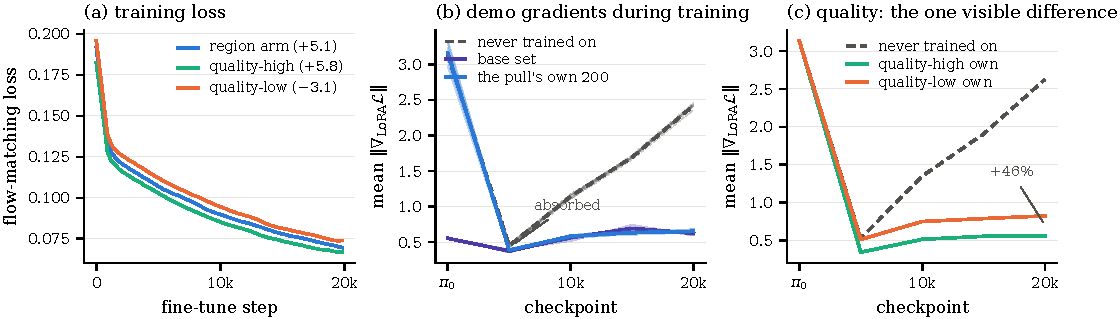
\includegraphics[width=\linewidth]{grad_three_panel.pdf}  % rendered 2026-08-14 by
  % gradient_analysis/make_paper_figure.py (7.0x2.35in, 8pt, Type-42 fonts)
  \caption{\textbf{The loss sees how a demonstration is executed, not what is in
  the scene.} \emph{(a)} Fine-tuning loss for the best and the worst pull of the
  study ($+7.8$ and $-2.7$\,pp, same seed, different $200$-demonstration draws):
  the curves are superimposed, so the $10.5$\,pp outcome spread is invisible at
  training time. \emph{(b)} Mean per-demonstration LoRA gradient norm along a
  fine-tune, for the pull's own draw, for $100$ never-trained pool
  demonstrations, and for the always-trained base set (6 trajectories,
  4 checkpoints, 360 demonstrations each). Own-draw norms collapse from
  $\approx$$3.2$ to $\approx$$0.4$ by step $5000$ and stay there---the
  demonstrations are fully absorbed, so the unmoved failure region reflects
  missing content, not under-training---while control norms climb back toward
  the pre-fine-tune level over the remaining $15{,}000$ steps, the signature of
  a recipe specializing to its particular draw. \emph{(c)} Per-demonstration
  gradient norm at the branching checkpoint for the top ($n{=}436$) and bottom
  ($n{=}439$) execution-quality tails: the distributions separate at AUC
  $0.719$ (norm alone; $0.778$ combining norm and a held-out quality direction),
  whereas the same statistics separate the diagnosed \emph{failure region} at
  $0.572$--$0.577$, at or below their label-shuffled null floor of
  $\approx$$0.60$ (dashed). Panels (b) and (c) are the same measurement applied
  to two different labelings of the same demonstrations---which is the
  section's argument in one figure.}
  \label{fig:grad_three_panel}
\end{figure}

\begin{table}[t]
\centering
\caption{Gate scores: is the target distinction encoded in the training
gradient? Best-mode AUC maximizes over SVD directions and must be read against
its own label-shuffled null floor (given in brackets). Sample sizes are
demonstrations (robot) or examples (sandbox).}
\label{tab:gates}
\setlength{\tabcolsep}{4pt}
\begin{tabular}{llcc}
\toprule
Loss / target & $n$ & Best mode [null] & Split-half \\
\midrule
CE / class (sandbox)          & --   & 0.66 [--]        & 0.870 \\
Flow / failure region         & 240  & 0.577 [0.598]    & 0.572 \\
Flow / region, mid-training   & 240  & 0.58--0.62 [$\approx$0.59] & 0.54--0.59 \\
\textbf{Flow / exec.\ quality} & 875 & \textbf{0.664} [0.589] & \textbf{0.663} \\
\bottomrule
\end{tabular}
% NOTE: the sandbox row's split-half 0.870 and target-direction 0.961 are now VERIFIED --
% reproduced 2026-08-14 by gradient_analysis/cifar_gate.py -> cifar_gate_report.json
% (same statistics code as the robot gate; ckpt 6000, 120v120, seed 20260730). Prior note kept:
% originally flagged UNVERIFIED in
% \S\ref{sec:grad_q4}; its best-mode 0.66 is attested.  The quality row's
% held-out combined score (norm + direction) is 0.778, reported in text.
\end{table}

\subsection{Relation to prior work}
\label{sec:grad_related}
Gradient-influence selection---LESS~\cite{less}, TracIn~\cite{tracin}---and
bandit-style extensions that use an influence proxy as a cheap reward, notably
ClusterUCB~\cite{clusterucb}, all presume that the training gradient encodes the
distinction being selected on. That premise holds for cross-entropy
instruction tuning, where the label is the regression target, and we measure it
false here: the premise is not a modeling detail but the load-bearing
assumption, and it is checkable in a few GPU-minutes before any fine-tune is
launched. CUPID~\cite{cupid} responds to the same problem from the other
direction, attributing closed-loop \emph{return} from evaluation rollouts rather
than training loss---which by construction sidesteps the encoding gate, at the
cost of requiring rollouts. Independently, D-TRAK~\cite{dtrak} reports that
training-loss gradients attribute poorly for diffusion models, and that
alternatives outperform the theoretically motivated loss-gradient
attribution---evidence that this is a property of denoising-style objectives
rather than a quirk of our task. Our contribution here is the gate itself as a
pre-flight check, the positive control that separates ``the loss cannot see it''
from ``the experiment cannot resolve it,'' and the observation that the axis the
robot loss \emph{does} encode is execution quality.
% CITATION STATUS:
%   \cite{less}, \cite{tracin}  -- VERIFIED, already in refs.bib.
%   \cite{cupid}   -- NOT in refs.bib.  Details cross-checked against
%                     weakregion/READING_LIST.md (Agia, Sinha, ..., Bohg;
%                     arXiv:2506.19121; CoRL 2025).  Add the entry.
%   \cite{clusterucb} -- UNVERIFIED.  arXiv:2506.10288 was supplied for this
%                     draft; NOT found in refs.bib and NOT in READING_LIST.md.
%                     Confirm authors/venue/title before submitting.
%   \cite{dtrak}   -- UNVERIFIED.  "D-TRAK", Zheng et al., ICLR 2024 was supplied
%                     for this draft; NOT in refs.bib, NOT in READING_LIST.md.
%                     Confirm exact title/authors/arXiv id.
% Suggested stubs (fill in the UNVERIFIED fields):
% @inproceedings{clusterucb,
%   title = {{ClusterUCB}: ...}, author = {...},
%   booktitle = {...}, year = {2025}, note = {arXiv:2506.10288}}
% @inproceedings{cupid,
%   title = {{CUPID}: Curating Data your Robot Loves with Influence Functions},
%   author = {Agia, Christopher and Sinha, Rohan and others and Bohg, Jeannette},
%   booktitle = {Conference on Robot Learning (CoRL)}, year = {2025},
%   note = {arXiv:2506.19121}}
% @inproceedings{dtrak,
%   title = {Intriguing Properties of Data Attribution on Diffusion Models},
%   author = {Zheng, Xiaosen and others},
%   booktitle = {International Conference on Learning Representations (ICLR)},
%   year = {2024}}

\subsection{Limitations}
\label{sec:grad_limits}
This diagnosis is one task (RoboCasa PickPlaceCounterToSink), one policy family
(a pi0 flow-matching VLA fine-tuned with LoRA), and one recipe ($20{,}000$
steps, batch $32$, $B{=}200$); we have not shown that the gate fails for other
VLA objectives, other tasks, or other budgets, only that the failure is a
property of what this objective regresses rather than of our design---which the
sandbox control establishes. The region labels being gated are themselves
model-derived (a frozen behavior map, held-out AUC $0.629$), and the quality
labels come from a heuristic execution score rather than ground truth, so both
gates measure encoding of a \emph{proxy} for the property of interest. Gradients
are estimated from $K{=}8$ frames per demonstration with single noise/time
draws and compressed to $2048$ dimensions, which attenuates all cosines
uniformly.

The deepest limitation is the one the whole program shares: every gate is a
\emph{loss-level} measurement, while the quantity we care about is
\emph{closed-loop rollout success}, and there is no theory connecting the two.
A passing gate is necessary for gradient-based selection, not sufficient for a
deployment gain. We have direct evidence of the gap in our own results: the
whitening selector of \S\ref{sec:anticorr} achieved the best offline ranking
metrics in the study and was significantly \emph{worse} than random when
deployed. For the same reason, the execution-quality filter of
\S\ref{sec:grad_q6} is reported as a passing gate and an in-progress causal
test, not as a validated method.


%%%%%%%%%%%%%%%%%%%%%%%%%%%%%%%%%%%%%%%%%%%%%%%%%%%%%%%%%%%%%%%%%%%%%%%%%%%%%%%%
% NOT-YET-SUPPORTED CLAIMS -- read before submission
% ------------------------------------------------------------------------------
% Each item is something this section either states as pending, deliberately
% stops short of, or would be tempting to strengthen during editing.  The list is
% ordered by how much it would cost the paper if a reviewer pushed on it.
%
% 1. CAUSAL VALUE OF THE QUALITY FILTER (\S\ref{sec:grad_q6}).  The gate passes
%    (AUC 0.719 / 0.778, n=875), but the causal arm test is NOT DONE: as of
%    2026-08-14 the ledger has NO gradqual_hi_j3 / gradqual_lo_j3 rows (55 pull
%    rows, none matching "gradqual").  Driver and frozen assignment exist
%    (gradient_analysis/gradqual_driver.py, gradqual_assignment.json; paired seed
%    1003, B=200, style-arm demos excluded so it is an independent selection).
%    Until those two rows land, do not write "filtering on gradient quality
%    improves success."  Pre-registered read is in gradqual_analyze.py.
%
% 2. TRANSFER OF THE FILTER TO NEW DATA SOURCES.  The section calls the filter
%    applicable to "simulation, an autonomous collector, or human teleoperation
%    on the G1."  That is an argument from mechanism, not a measurement: the gate
%    was only ever run in-pool, on MimicGen demonstrations of this one task, at
%    this one checkpoint.  Nothing has been gated on G1 or GR00T data.  Soften to
%    "should transfer in principle" unless a G1 gate run lands.
%
% 3. STYLE / QUALITY RACE SIGNIFICANCE.  high-low = +8.9/+2.9/+2.9 pp, mean +4.9,
%    3/3 consistent in sign, but one pull per arm per round against
%    sigma_e = 3.3 pp.  It is DIRECTIONAL.  The draft says so; keep it that way.
%    Same for the Q2c absorption difference (0.83 vs 0.57) -- one pull per arm.
%
% 4. EARLY STOPPING AS A NOISE REMEDY.  \S\ref{sec:grad_q2} notes late-training
%    specialization is a "plausible amplifier" of pull noise and explicitly does
%    not claim the remedy works.  A training-length ablation DOES exist in the
%    ledger (ablate_{mid_band,random}_j5_ck{10000,15000}, 450 eval episodes each)
%    and the handoff says the 10k-vs-20k duration question was answered, but no
%    report under gradient_analysis/ analyzes it, so its result is unknown to
%    this draft.  Do NOT upgrade the sentence to a recipe recommendation without
%    pulling those numbers.
%
% 5. CIFAR GATE SCORES 0.870 / 0.961.  Supplied for this draft; NOT found in
%    xgradtest/ or gradient_analysis/ artifacts.  Attested nearby numbers:
%    influence AUC 0.96 (cosine variant 0.958) and best-single-mode 0.66.
%    Either locate the run that produced 0.870/0.961 or replace the table row
%    and the sentence in \S\ref{sec:grad_q4} with the attested figures.
%
% 6. SAME-DATA/DIFFERENT-SEED COSINE 0.505 (\S\ref{sec:grad_q5}).  Computed from
%    the single available such pair (the two null pulls).  n=1 pair.  A second
%    null pair at a new seed would cost one fine-tune and make the paragraph
%    airtight; without it, phrase as "the one available pair."
%
% 7. WEIGHT-SPACE ORTHOGONALITY (\S\ref{sec:grad_q5}).  cos(-G, dtheta) <= 0.03
%    is only safe as a within-family comparison: the leaf-ordering match between
%    gradient flattening and parameter flattening was never independently
%    verified.  If a reviewer asks "did you check the flatten order?", the honest
%    answer today is no.  Either verify it or drop that sentence.
%
% 8. GENERALITY OF THE ENCODING FAILURE.  The paper will want to say "the
%    flow-matching loss does not encode scene semantics."  What is measured is:
%    one region definition (behavior-descriptor cluster) and, earlier, one object
%    -category definition, on one task, one policy.  D-TRAK is cited as
%    independent support for denoising objectives -- and that citation is itself
%    UNVERIFIED (item 10).  Keep the claim scoped to "this objective on this
%    task" in every sentence that a reviewer could quote out of context.
%
% 9. B=200 ONLY.  "Selection from a fixed pool is closed by mechanism" is
%    established at one budget.  The exchangeability argument (region cosine 0.024
%    vs 0.019 against a common mode of 0.20) is budget-independent in spirit, but
%    no larger or smaller B was run.  Say "at this budget" at least once.
%
% 10. CITATIONS.  clusterucb (arXiv 2506.10288) and dtrak (Zheng et al., ICLR
%     2024) are UNVERIFIED -- absent from refs.bib AND from the project's own
%     verified sweep in weakregion/READING_LIST.md.  cupid (arXiv 2506.19121) is
%     verified in READING_LIST.md but has no refs.bib entry yet.  All three need
%     entries added before this section compiles cleanly.
%
% 11. RECONCILIATION WITH \S4.4 OF main.tex.  \S4.4 currently reports a CIFAR
%     influence AUC of "~0.96" and a RoboCasa category ceiling of "~0.60" as the
%     gradient-encoding argument.  This section reports the same principle with
%     different, region-based numbers.  Two different sets of gate numbers for
%     "the same" claim in one paper invites a reviewer to ask which is the
%     result.  Decide on one primary presentation.
%%%%%%%%%%%%%%%%%%%%%%%%%%%%%%%%%%%%%%%%%%%%%%%%%%%%%%%%%%%%%%%%%%%%%%%%%%%%%%%%
